% Chapter 12

\chapter{Análisis y Resultados} % Chapter title

\label{ch:analisis_resutados} % For referencing the chapter elsewhere, use \autoref{ch:name} 

%----------------------------------------------------------------------------------------
\section{Prototipo CWC}
El prototipo de CWC se programó utilizando el lenguaje de programación Python. Además se utilizó una biblioteca llamada btpeer. Esta biblioteca implemente un protocolo P2P, el cual permite el intercambio de archivos. En la figura \ref{cwc} se pude ver la interfaz prototipo para un cliente-servidor.

\begin{figure}[h]
  \centering
    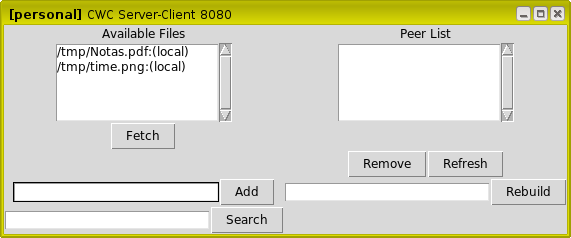
\includegraphics[scale=0.75]{gfx/cwc}
  \caption{Prototipo de CWC}
  \label{cwc}
\end{figure}

\section{Resultados de Rendimiento}

\begin{table}[h] %here h, t top, b bottom, p dedicated page on floats
\myfloatalign
\begin{tabular}{lcccc} \toprule % four columns, fist left, other ones centered. 
\tableheadline{Tipo de Archivo} & \tableheadline{Tamaño (MB)} & \tableheadline{Servidor Web} \\ \midrule
Imágenes & 2.4 & 12.6 s \\ 
Videos & 345.9 & 1802.1 s  \\
Documentos & 1.3 & 6.6s  \\
Instaladores & 34.6 & 181.2s  \\
\end{tabular}
\caption{Resultados del escenario Sin Web Caché}  
\label{tab:crecimiento_internet}
\end{table}

\begin{table}[h] %here h, t top, b bottom, p dedicated page on floats
\myfloatalign
\begin{tabular}{lcccc} \toprule % four columns, fist left, other ones centered. 
\tableheadline{Tipo de Archivo} & \tableheadline{Tamaño (MB)} & \tableheadline{1 Nodo} & \tableheadline{2 nodos} & \tableheadline{3 nodos}\\ \midrule
Imágenes & 2.4  & 13.4 s & 12.9 & 13.1 \\ 
Videos & 345.9 & 1786.5 &  & 902.8 s & 603.7 s \\
Documentos & 1.3 & 7.1 s & 6.9 & 7.0 s \\
Instaladores & 34.6 & 168.4 s & 88.57 & 58.2 s \\
\end{tabular}
\caption{Resultados del escenario Prototipo CWC}  
\label{tab:crecimiento_internet}
\end{table}

\section{Análisis de rendimiento de velocidad del entorno de CWC}

Las herramienta seleccionada para la medición del rendimiento fueron:
\begin{itemize}
\item Httperf: Se utilizó para medir el rendimiento del escenario Sin Web Caché
\item time: Se utilizó para medir el rendimiento del escenario del prototipo de CWC
\end{itemize}

\section{Resultados de Costo}

%----------------------------------------------------------------------------------------

\section{Análisis de costos del Entorno de CW}

Content